\documentclass[aspectratio=1610,xcolor=dvipsnames,t]{beamer} 

\usepackage{listings} 
\usepackage{color} 
\usepackage{xcolor}  
\usepackage{microtype} 
\usepackage{helvet} 
\usepackage{inconsolata} 
\usepackage[framemethod=TikZ]{mdframed} 
\usepackage{graphicx} 
\usepackage{alltt}
\usepackage{sverb} 
\usepackage{verbatim} 
\usepackage{pifont} 
\usepackage{helvet} 
\usepackage{algorithm}
\usepackage{algpseudocode}

\usetheme{Madrid} 
\useinnertheme{rectangles} 

\setbeamertemplate{navigation symbols}{}
\setbeamertemplate{blocks}[default] 

%\definecolor{mypurple}{rgb}{.49,0,98}
%\setbeamercolor*{palette primary}{use=structure,fg=white,bg=green}
%\usecolortheme[rgb={0.9,0.2,0.2}]{structure}
%\usecolortheme[rgb={0.6,0.1,0.1}]{structure}

%\usecolortheme[rgb={0.2, 0.2, 0.8}]{structure} 
%\usecolortheme[rgb={0.0, 0.0, 0.8}]{structure} 
\usecolortheme[rgb={0.2, 0.2, 0.3}]{structure} 

\usepackage{color}
\definecolor{orange}{cmyk}{0,0.4,0.8,0.2}
\definecolor{darkorange}{rgb}{.71,0.21,0.01}
\definecolor{darkgreen}{rgb}{.12,.54,.11}
\definecolor{myteal}{rgb}{.26, .44, .56}
\definecolor{gray}{gray}{0.45}
\definecolor{lightgray}{gray}{.95}
\definecolor{mediumgray}{gray}{.8}
\definecolor{inputbackground}{rgb}{.95, .95, .85}
\definecolor{outputbackground}{rgb}{.95, .95, .95}
\definecolor{traceback}{rgb}{1, .95, .95}
\definecolor{inputbg}{rgb}{0.98, 0.98, 0.98}

\usepackage{listings} 
\lstset{language=bash,
        %basicstyle=\footnotesize\ttfamily, 
        basicstyle=\small\ttfamily,
        columns=fullflexible, 
        %title=\lstname, 
        %numbers=left, stringstyle=\texttt, 
        %numberstyle={\tiny\texttt}, 
        keywordstyle=\color{blue}, 
        commentstyle=\color{darkgreen}, 
        stringstyle=\color{purple} } 


\mdfsetup{skipabove=\topskip, skipbelow=\topskip} 

\definecolor{codebg}{rgb}{0.99,0.99,0.99}

\global\mdfdefinestyle{code}{%
    frametitlerule=true,%
    frametitlefont=\small\bfseries\ttfamily,%
    frametitlebackgroundcolor=lightgray,%
    backgroundcolor=codebg,%
    linecolor=gray, linewidth=0.5pt,%
    leftmargin=0.5cm, rightmargin=0.5cm,%
    roundcorner=2pt,%
    innerleftmargin=5pt
}

\global\mdfdefinestyle{code2}{%
    topline=false,%
    bottomline=false,%
    leftline=true,%
    rightline=false,%
    backgroundcolor=codebg,%
    linecolor=gray, linewidth=0.5pt,%
    leftmargin=0.0cm, rightmargin=0.0cm,%
    innerleftmargin=1pt
}

\newcommand{\showcode}[1]{\begin{mdframed}[style=code] %
                            \lstinputlisting{#1}% 
                          \end{mdframed}% 
}


\title[Intelligent Virtual Environments]{Intelligent Virtual Environments for Agents} 
\subtitle{2002 Australian Cognitive Science Conference} 
\author[Michael Papasimeon]{Michael Papasimeon} 
\date[OZCOGSCI 2002]{25 September 2002\\ Fremantle, Western Australia} 

\begin{document}

\begin{frame}
    \maketitle
\end{frame} 

\begin{frame}{Overall Aim and Hypothesis} 
    \begin{block}{Aim}
        To allow agents to participate in a richer, more complex and more
        intelligent way in their environment in the framework of an explainable
        and plausible cognitive model. 
    \end{block}
    \begin{block}{Hypothesis}
        \begin{itemize}
            \item Current agents are limited by their environmental
                  interaction.
            \item We can attempt to change this by improving the way
                  in which agents interact with their environment.
        \end{itemize}
    \end{block} 
    \begin{exampleblock}{Herb Simon (1969)} 
        \begin{quote}
            "Complexity of an ant's behaviour walking along a beach
            has more to do with the complexity of the environment
            rather than an inherent internal complexity of the 
            ant itself."
        \end{quote}
    \end{exampleblock} 
\end{frame} 

\begin{frame}{Definitions: Agent} 
    \begin{block}{Russell and Norvig \emph{Artificial Intellligence -- pg 31, 1995}}
        \begin{quote}
            "An agent is anything that can be viewed as perceiving its 
            \textbf{environment} through sensors and acting upon that
            \textbf{environment} through effectors."
        \end{quote}
    \end{block} 

    \begin{block}{d'Inverno and Luck \emph{Understanding Agent Systems -- pg 2, 2001}}
        \begin{quote}
            "... agents have been proposed as \textbf{situated} and 
            \textbf{embedded} problem solvers that are capable of functioning
            effectively and efficiently in a complex \textbf{environment}."
         \end{quote} 
    \end{block} 

    \begin{block}{Wooldrdige \emph{Multiagent Systems - pg 29, 1999 - editor G. Weiss}}
        \begin{quote}
            "An agent is a computer system that is \textbf{situated} in some
            \textbf{environment} and that is capable of autonomous 
            \textbf{action} in this environment in order to meet its
            design objectives."
        \end{quote}
    \end{block} 

\end{frame} 

\begin{frame}{Definition: Environment}
    \begin{itemize}
        \item Agents can be situated in different types
              of environments:
              \begin{itemize}
                    \item Real
                    \item Virtual
              \end{itemize}
        \item We are interested in synthetic (spatial and temporal)
              environments that are representations of real
              or fictional worlds:
                \begin{itemize}
                    \item Simulations
                    \item Interactive Entertainment
                \end{itemize}
    \end{itemize}
    \begin{center}
        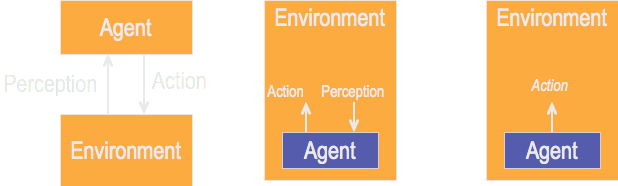
\includegraphics[width=0.8\textwidth]{environments} 
    \end{center}
\end{frame} 

\begin{frame}{Requirement for Virtual Environments} 
\end{frame} 

\begin{frame}{Definition: Intelligent}
    \begin{itemize}
        \item ...as in Artificial Intelligence.
        \item Including perception, reasoning and action.
        \item Components of a software system that contains "smarts":
            \begin{itemize}
                \item Components which use traditional AI algorithms
                \item Components which are models of human cognitive 
                      processes.
            \end{itemize}
        \item Research in multi-agent systems suggest that these
              types of processes belong in the agent. 
    \end{itemize}
\end{frame} 

\begin{frame}{Designing Intelligent Information Systems} 
    \begin{itemize}
        \item Limited representation of the environment in classical
              artificial intelligence.
        \item Then agents came along... agent could live in,
              perceive, reason and act in their environment.
        \item Many agents became quite large and heavyweight and
              exhibit properties of classical AI systems.
        \item "Intelligence" belongs in the agent?
    \end{itemize}
    \begin{center}
        
\includegraphics[width=0.8\textwidth]{intel-spectrum} \\
        The software design spectrum -- where to put the intelligence in an
        intelligent system?
    \end{center}
\end{frame}

\begin{frame}{Real Environments: Augmentation} 
    Augmenting real environments for a purpose
    \begin{itemize}
        \item Head Up Displays and Helmet Mounted Sights
        \item The Road and Traffic System
    \end{itemize}
\end{frame} 

\begin{frame}{Classical AI vs Situated Cognition}
    \begin{block}{Classical AI vs Situated Cognition}
    \begin{center}
    \begin{tabular}{cc} \hline
        \textbf{Classical View of Mind}  &   \textbf{Situated Cognition} \\ \hline
            Individual              &   Social \\
            Rational                &   Embodied \\
            Abstract                &   Concrete \\
            Detached                &   Located \\
            General                 &   Specific \\ \hline
    \end{tabular} 
    \end{center} 
    \end{block} 

    It is claimed that agents are situated given that they
    can perceive and act in an environment. However:
    \begin{itemize}
        \item Most agent designs don't have the characteristics
            espoused by the situated cognition community.
        \item Most agent designs ignore the environment and are
            detached (reasoning is separate from perception and action).
    \end{itemize}
            

\end{frame} 

\begin{frame}{Ideas for Designing Virtual Environments}
    \begin{itemize}
        \item Situated Cognition (Clancy, Suchman)
        \item Cognitve Systems (Hutchence) -- Boeing 747 Example
        \item Ecological Psychology (Gibson) -- Affordances
        \item Labelling of Entities in the Environment by:
            \begin{itemize}
                \item Name, Category
                \item Affordance
                \item Relationships
                \item Purpose or Intention of Agens
            \end{itemize}
    \end{itemize}
    
    Consider a motor racing simulation/game...
\end{frame}

\begin{frame}{Motor Racing Simulation: The Scenario}
\end{frame} 

\begin{frame}{Environmental Representation Options} 
    \begin{itemize}
        \item Agent driving a virtual car around a virtual racing track...
        \item The environment consists of a track, other cars,
              obstacles, team-mates, marshals, the pits, pit-crew,
              team-boss, spectators.
        \item What our virtual environment representation options?
            \begin{itemize}
                \item Intelligent Agents
                \item Intelligent Environments
                \item "Intelligence" is shared between agents and environments.
            \end{itemize}
    \end{itemize}
\end{frame} 

\begin{frame}{Intelligent Agent: Low Level Perception}
    \begin{itemize}
        \item One extreme is to make the agent do everything starting 
              with low level perception…
        \item Agent needs to perceive geometry, colour, lighting, material, 
              motion and then recognise high level objects such as roads etc.
        \item \textbf{Advantage:} agent is portable to many types of environments.
        \item \textbf{Disadvantage:} computationally expensive, a lot of 
               engineering is spent designing low level processing.
    \end{itemize}
\end{frame} 

\begin{frame}{An Environment Labelled for an Agent}
\end{frame} 

\begin{frame}{Driver Agent: Rounding a Corner}
\end{frame} 

\begin{frame}{Labels, Names, Categories and Plans}
    \begin{itemize}
        \item We can label things in different ways.
            \begin{itemize}
                \item As cars, roads, buildings, traffic lights.
                \item As opponents, pedestrians and other drivers, 
                      or everything is an obstacle to the 
                      agent winning!
            \end{itemize}
        \item Parts of the environment can be labelled. 
              For example, consider labelling a corner:
              \begin{itemize}
                    \item As a left/right tight turn
                    \item With prescription: \emph{"Take this corner
                            at 60-75 km/h, in 3rd gear in a gentle
                        left hand turn."} 
              \end{itemize}
    \end{itemize}
\end{frame} 

\begin{frame}{Environmental Labelling by Category} 
\end{frame}

\begin{frame}{Relationships in the Environment}
    \begin{itemize}
        \item Can the agent driver query the environmnet about 
              relationships?
              \begin{itemize}
                \item \emph{"Who is in front of me?"}
                \item \emph{"Who is behind me?"} 
              \end{itemize}
        \item How about more complex relationships that are dynamic?
            \begin{itemize}
                \item \emph{"Do I have an overtaking opportunity?"}
            \end{itemize}
        \item Relationships between team members.
    \end{itemize}
\end{frame}

\begin{frame}{Affordances in Crazy Taxi} 
    \begin{itemize}
        \item Premise is to pickup fare paying passengers.
        \item The quickest route to the destination, the more
              money the passenger will pay.
        \item Passengers tip extra for crazy stunts and tricks.
        \item Certain buildings afford picking up passengers.
        \item Objects in the the city afford doing stunts 
              (like ramps for jumps).
        \item Different road surfaces afford going faster.
        \item All sorts of things afford being a short-cut.
    \end{itemize}
\end{frame} 

\begin{frame}{An Environment Labelled for an Agent} 
\end{frame} 

\begin{frame}{Summary}
    \begin{itemize}
        \item Agent interactions with the environment aren't
              as interesting or complicated as they could be.
        \item Virtual environments and agents can be designed
              (unlike real environments).
        \item Exploring the "agent-environment" interface allows
              us to investigate alternative ways of intelligent
              agents in virtual environments.
        \item We can use ideas from cognitive science to  
              ground our designs in theory of situated cognition.
        \item This will help us build environments in which agents
              and humans can interact. 
    \end{itemize}
\end{frame} 


\end{document}
